\pattern{Strategy}
\begin{summary}
    The {\bf Strategy} pattern resembles a {\bf State} pattern but it
    encapsulates algorithms instead of data. 
    
    % TODO what does this mean
    You can see that the Context class in the Strategy Class Model is an
    (aggregator) has a Strategy interface (aggregate).
\end{summary}

\comparison{\begin{itemize}
        \item Flexibility: a solution to a problem can use many options and it
            is easy to apply the selected algorithm. Users can choose the most
            suitable algorithm for their systems. 
        \item High encapsultation: it is easy to add, remove, or switch algorithms
            because each strategy is encapsulated into separate classes.
            Changing one algorithm does not affect the others. Additionally, 
            each algorithm can be tested independently.
        \item Loosely coupled: algorithms are not reliant on each other within the
            context entity. They can be changed or replaced without changing the
            context entity.
        \item Readability: the pattern reduces the number of conditional
            statements such as if-else statements or switch statements. Conditionals can
            be computationally expensive.
        \item Reusability: Algorithms and behaviours can be easily reused, due
            to their high level of encapuslation.
    \end{itemize}

}{\begin{itemize}
        \item Prior knowledge about each algorithm is required. Users must know
            about various strategies/algorithms to select the best one for
            them.
        \item Performance: It increases the number of objects in the application.
            a. It requires many objects to do its job, which increases memory requirements.
            b. It may cause an impact on performance of the application.

    \end{itemize}
} % END comparison

\begin{nfps}
\item[Maintainability] It is easy to modify or replace algorithms, which can be
    done in separate classes.
\item[Testability] Since each algorithm is encapsulated into separate classes,
    it allows developers test each algorithm separately. This is less complex
    and tends to be more reliable.
\item[Extensibility] When users need new algorithms, it is easy to add them
    since it can be done by creating new strategy classes. This creation
    process does not affect other algorithms.
\item[Reusability] Algorithms and behaviours can be easily reused because they
    are encapsulated.
\end{nfps}

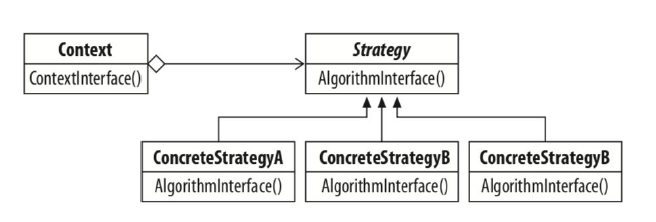
\includegraphics[width=0.5\textwidth]{./strategy}
